	% %%%%%%%%%%%%%%%%%%%%%%%%%%%%%%%%%%%%
% A LaTeX template for the technical essay of TTM4137 Wireless Security
% Stig F. Mjolsnes, 01.09.2012
%%%%%%%%%%%%%%%%%%%%%%%%%%%%%%%%%%%%%
\documentclass[a4paper,11pt]{article}

\usepackage[plain]{fullpage}
\usepackage{graphicx}  %This enables the inclusion of pdf graphic files in figures
\usepackage{hyperref} % Make links in your document click-able NB: must be loaded before the caption-package
\usepackage{caption}
\usepackage{subcaption}
\usepackage{wrapfig}
\usepackage{sidecap}
\usepackage[utf8]{inputenc}


\title{Attacks on Near Field Communications on Mobile Phones}
\author{Håkon Nymo Matland \\
	\texttt{hakonnym@stud.ntnu.no}\\
	TTM4137 Wireless Security Technical Essay}
\date{\today}

\begin{document}
\maketitle


\section{Introduction}
The Near Field Communication (NFC) technology is being deployed in mobile phones all over the world. The technology's applications is wide, covering authentication, file sharing, and perhaps the most promising application: payment solutions using NFC~\cite{remedios2006nfc}~\cite{tan2013}. An analysis by Berg Insight claim that one in three mobile phones will come with NFC by 2017~\cite{nfc_growth}, making the technology a huge future marked.

\paragraph{}NFC is a set of standards for devices to establish radio communication with each other by bringing them in close proximity, usually not more then a few centimeters. NFC standards cover communications protocols and data exchange formats, and was highly influenced by the RFID standard. Communication is possible between two NFC enabled devices, or a NFC enabled device and unpowered electronic chips.


\paragraph{}The need of security and robustness is very important, as an insecure and attackable device would give criminals new ways to steal funds, or simply take control over the device. Different attacks have been proven successful and malicious, and the threat should be taken seriously by both individuals and corporations. Simple RFID-stickers and vulnerabilities in software is all an attacker need to do harm. This essay will present and discuss some of the successful or potential attacks previously demonstrated by experts in the field of NFC and security.


\section{Problem discussion}

\subsection{Eavesdropping}
As with every other wireless communication interface eavesdropping is an obvious threat. If the communication is not properly encrypted and secured, parties not participating in the transmission of data may capture the radio frequencies and store them for analysis. Some sites use the requirement for close proximity, and the possibility of secure channels as arguments that eavesdropping is not an issue~\cite{nfceaves}. An experiment as part of the master thesis by Henning Siitonen Kortvedt at the Norwegian University of Science and Technology concluded that it is practical possible to capture and demodulate data sent in both directions between two NFC interfaces~\cite{kortvedt2009eavesdropping}~\cite{kortvedt2009securing}. If the data communicated is not correctly secured, the threat of eavesdropping is quite clear. No services benefit from giving illegitimate third parties the opportunity to eavesdrop on the communication of the service.


\subsection{Smart poster URI spoofing}

With the deployment of NFC capable mobile phone, the concept of smart posters came.
The poster is used to advertise or give the customer a service. The user only has to tap their NFC enabled mobile phone in close proximity to the advertisement, and something happens on the phone~\cite{ruiz2009university}~\cite{smartposter}. Through social engineering or software vulnerabilities this can be exploited. Changing the RFID chip in the poster makes it possible for customers to believe they are accessing a legitimate service, while they are not. 

\subsubsection{Web browser exploits and malicious software download}

A possible scenario is an user tapping their phone on a smart poster to gain the URL of a service. If an attacker has changed the RFID chip to one of his own, he can trick the users to enter a spoofed URL, with the goal of phishing sensitive information through a login or sign up form. 

\begin{wrapfigure}[11]{R}{0.450\textwidth}
  \vspace{0cm}
  \centering
  \vspace{-1cm}
  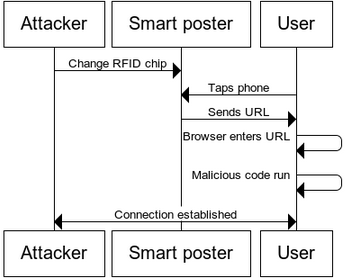
\includegraphics[scale=0.5]{SD_SmartPoster1} %Note: no use of .jpg file ending
  \vspace{-0.4cm}
  \caption{Smart poster attack
  \label{fig:SD_SmartPoster1}}
\end{wrapfigure}
In 2012 security researcher Charlie Miller proved how he with a simple RFID sticker could gain full root shell access on an Android phone~\cite{cmiller}~\cite{cmiller1}. With full root shell access, several exploits are possible. Charlie miller was able to download every file on the device. Although the attack primarily used exploitable bugs in the browser, the attack was triggered by the NFC interface of the device.

\paragraph{}
The concept described above can also be used more explicitly to run malicious code on the device. The attacker has the possibility to trick the user into downloading an application to install directly. On Android devices you could simply use the smart poster to direct the user to a .apk file on the internet. If the poster is trying to advertise an app, a user not thinking critically might install the fake application, and make the device send all kind of data to the attacker. The application may appear like the one the user wanted to download, with a similar name and icon.

\subsubsection{Premium rated telephone services}

Similar to have a RFID chip send a web URL, it can also be used to invoke telephone connections or sending SMS~\cite{mulliner2009vulnerability}. The user might be asked if he wants to call or send, but some users will likely not pay attention to what is says on the screen if it is received from what looks to be a legitimate source. This opens a whole new range of premium service rate scams. A poster claiming to let you call a free service might suddenly make an user call an expensive premium rate number. A user trying to purchase something from a vending machine might end up with a high phone bill, and no snack. The idea may even be mixed together with a man-in-the-middle attack, by using the premium rate service number as a proxy towards the legitimate service. Many users would not even notice that the chocolate bar they bought was charged more than the price listed on the vending machine.


\subsection{Denial-of-Service attacks}
A Denial-of-service attack(DoS attack) is an attempt to make a service unavailable to its intended users. The motivation for an attacker to perform a DoS attack may vary, but the result is nonetheless destructive. DoS attacks may be used to destroy the trust relationship between the customer and the service provider, or simply to conduct mischief. NFC services may be denied by creating distortion of the signals, or by invoking unwanted effects as rebooting. The smart poster range of attacks may also serve as Denial-of-Service attacks.

\subsubsection{Dirty use of USSD and MMI codes}
Unstructured Supplementary Service Data (USSD) is a protocol used by GSM cellular telephones to communicate with the service provider's computers. Some device manufacturers have also implemented their own set of codes similar to USSD, called MMI to make changes to the device or view/test settings. Several devices also have MMI codes to reboot the device, or even factory reset the device.

In 2012 security expert Ravi Borgaonkar showed how MMI codes transmitted with NFC could be used to run a full factory reset on newer Samsung devices~\cite{USSD}. Borgaonkar used NFC to make a Samsung Galaxy S3 do a full factory reset by making it dial the MMI code *2767*3855\#. The exploit was possible to invoke not only with NFC, but also through QR-codes and code hidden within frames on web pages. The code implemented by Samsung did not ask for a confirmation, nor gave any way to stop the process. The device attacked would loose all locally stored data. Consider the consequences of this attack mixed with a smart poster chip swap at a busy subway station. Other codes can be used to lock the sim card, and even make it useless.

\section{Conclusion}
This essay has talked briefly about some of the possible threats emerging together with NFC.

Eavesdropping is not a concern if encryption algorithms are correctly implemented, but as NFC grows to be a widely used technology, there will be implementations not done correctly with possible exploits as a result. Communication done in payment solutions will be implemented with great cryptographic algorithms and should not be threaten by eavesdropping.

The different attacks made through NFC smart posters show how scammers and criminals can exploit the naive smart phone users. Through appearing like legitimate services, scammers can claim control over devices, steal log in information or make them call expensive premium rate numbers. The best way to defend against these kind of attacks is to be sceptical to the information received from tags. Is the number appearing on your phone match the one on the poster? The idea of just "tapping" the phone to make something happen may even make the end user more naive, and an even easier target to scam.

\paragraph{}
Old technologies, ideas and principles can also be affected by the new possible ways of transmitting data. The Samsung USSD/MMI attack showed how critical implementation of old technologies become when mixed with NFC. New possibilities are found, not only by the device manufacturers, but also attackers looking for new ways to scam and trick people.

Many of the attacks on NFC is based on tricking the user. It's not necessarily technological flaws, but flaws in the mind of the users. Many users will not think about the possibility that an tag has been swapped, or that they can be subject to man-in-the-middle attacks at a vending machine.

It is important to notice that many of the attacks described above has been software exploits, and not directly the NFC interface not secured properly. High scale attacks can be avoided if software developers are quick to patch and update their product. However, there is a large number of devices out there running on old software, with no intention of being updated.


\newpage{}

% It is highly recommended to keep your references in a separate file (here called "references.bib")
% However if you want to create the reference section manually, 
% uncomment the lines below starting at "\begin{thebibliography} ... etc"
\bibliographystyle{unsrt}
\bibliography{references}\label{sec:references}



%\begin{thebibliography}{N}\label{sec:references}
%\bibitem{wiki1} Wikipedia. \textit{Citation.} Available at \url{http://en.wikipedia.org/wiki/Citation}.
%
%\bibitem{Daborn} Gordon Baxter, Jon Lewis and Ishbel Duncan. \textit{What is a Technical Essay?}
%Available online at \url{http://ishbel.host.cs.st-andrews.ac.uk/WhatisaTechnicalEssay.pdf}.
%
%\bibitem{Kortvedt} Henning Kortvedt and Stig Frode Mj{\o}lsnes. \textit{Eavesdropping Near Field Communication}.  
%In The Norwegian Information Security Conference (NISK 2009) Proceedings, pp. 57-68.  Tapir Akademiske Forlag, 2009.
%
%\end{thebibliography}  


\end{document} 
